\section{Extended Evaluation and Design Details}
\label{app:extended}

This appendix holds material that the main text refers to and that is not needed to follow its argument: tables, figures and analyses moved from the main sections, unchanged.

\subsection*{Safety evaluation: additional tables and the peripheral quorum gate}

\begin{table}[tbp]
\caption{Collusion suite at $n{=}7$ (A3 and A4 are the single-actor cases it
reruns; B8 is three runs of an honest split view with no adversary; c0 is the control)}
\label{tab:f2}
\centering
\scriptsize
\setlength{\tabcolsep}{3pt}
\resizebox{\linewidth}{!}{\begin{tabular}{@{}lrllrrr@{}}
\toprule
\textbf{Case} & \textbf{Byz.} & \textbf{Behaviour} & \textbf{Rejected by honest validators} & \textbf{Repeats} & \textbf{Same AppHash} & \textbf{Replay clean} \\
\midrule
a3 & 1 & claims a DA attestation one height ahead & none & 3 & 3/3 & 3/3 \\
a4 & 1 & forged Bitcoin checkpoint hash & btc verify receipt 216 & 3 & 3/3 & 3/3 \\
b1 & 2 & coordinated false degraded observations & none & 3 & 3/3 & 3/3 \\
b2 & 2 & false observations; proposer biases the certificate & none & 3 & 3/3 & 3/3 \\
b3a & 1 & proposer keeps exactly a quorum of certificates & none & 3 & 3/3 & 3/3 \\
b3b & 1 & proposer keeps fewer than a quorum & sub quorum certificate 210 & 3 & 3/3 & 3/3 \\
b4 & 2 & double-signing at the same height & none & 3 & 3/3 & 3/3 \\
b5 & 2 & withdrawal in a block of a locked state & withdrawal locked 320 & 3 & 3/3 & 3/3 \\
b6 & 2 & stale DA receipt; forged Bitcoin hash & btc verify receipt 155, da verify receipt 165 & 3 & 3/3 & 3/3 \\
b7a & 2 & false observations with two honest validators eclipsed & none & 3 & 3/3 & 3/3 \\
b7b & 2 & false observations with three honest validators eclipsed & none & 3 & 3/3 & 3/3 \\
b8 & 0 & honest split view: 3 then 4 of 7 eclipsed & none & 1 & 1/1 & 1/1 \\
c0 & 0 & control: node04 restarted, no behaviour & none & 3 & 3/3 & 3/3 \\
\bottomrule
\end{tabular}
}
\end{table}

The suite fixes the number of Byzantine validators; the threshold itself is
measured in a second sweep (Table~\ref{tab:b9}) with $b \in \{0,1,2,3\}$
validators and two adversary goals: forcing \textsc{Sovereign} through false degraded
observations, and hiding a real DA outage by reporting it healthy.
Each cell is five runs, each on a fresh chain started from \textsc{Anchored}. For $b \le 2$ no block lay outside
the honest range and the adversary reached neither goal (30 of 30 runs). For $b{=}3$ the aggregate left the honest range in 40--42 blocks and
the adversary forced \textsc{Sovereign} in 5 of 5 runs, which is the boundary Lemma~\ref{lem:honest-range}
predicts. Hiding an outage did not succeed at $b{=}3$ either: honest proposers' blocks
still reported it (5--12 blocks outside the range). An outage can be hidden only
when every run of consecutive honest proposers is shorter than the hysteresis threshold, and these
placements did not produce that.

\begin{table}[tbp]
\caption{Threshold sweep: Byzantine validators $b$ at $n{=}7$ ($f{=}2$)}
\label{tab:b9}
\centering
\scriptsize
\setlength{\tabcolsep}{3pt}
\resizebox{\linewidth}{!}{\begin{tabular}{@{}llrrrr@{}}
\toprule
\textbf{Goal of the adversary} & \textbf{Byz.} & \textbf{Runs} & \textbf{Blocks outside honest range} & \textbf{Same AppHash} & \textbf{Adversary's goal reached} \\
\midrule
force \textsc{Sovereign} & 0 & 5 & 0 & 5/5 & 0/5 \\
force \textsc{Sovereign} & 1 & 5 & 0 & 5/5 & 0/5 \\
force \textsc{Sovereign} & 2 & 5 & 0 & 5/5 & 0/5 \\
force \textsc{Sovereign} & 3 & 5 & 40--42 & 5/5 & 5/5 \\
hide a DA outage & 0 & 5 & 0 & 5/5 & 0/5 \\
hide a DA outage & 1 & 5 & 0 & 5/5 & 0/5 \\
hide a DA outage & 2 & 5 & 0 & 5/5 & 0/5 \\
hide a DA outage & 3 & 5 & 5--12 & 5/5 & 0/5 \\
\bottomrule
\end{tabular}
}
\end{table}


\textbf{Peripheral P2P quorum gate.} A P2P detector is useful for safety only if
its signal cannot be abused by a minority. A Monte Carlo sensitivity study on
synthetic attacks that we define shows that the six-bound profiler flags every
full-intensity snapshot and every ramp, reads attacks of low intensity (up to 0.25)
as healthy, and that a peer-count-only detector detects none of them
(Appendix~\ref{app:attacks}); it does not measure robustness against arbitrary
eclipse or Sybil strategies. We then ran the two most diagnostic attacks live.
In P3
(churn-based rotation: eight restart cycles on two of seven validators,
29\% of voting power), no FSM transition was committed in any of three runs (in
the first, the churn metric on both attacked validators crossed its threshold):
two validators' signed observations cannot move a certified aggregate backed by a
quorum. In P4 (a sustained delay of 350$\pm$50\,ms on all of one validator's P2P interfaces,
which all seven validators observe), the chain escalated in each of three runs on fresh chains: all
validators entered \textsc{Suspicious} 30--35\,s and \textsc{Sovereign} 60--66\,s after the delay began.
After the delay cleared, every run returned to \textsc{Anchored} at all seven validators, on average 279\,s later
(95\% interval $\pm$26\,s, Student $t$). The return is paced by the recovery proof that proof-only recovery with an unproven tail
of 128 blocks requires (Section~\ref{subsec:rq3}), not by the hysteresis waits; an earlier single trial with the heuristic fallback
returned within seconds (Fig.~\ref{fig:a4-cascade}). Each run also showed a brief fall-back from \textsc{Recovering} to \textsc{Sovereign}
(Section~\ref{subsec:limitations}).

\begin{figure}[tbp]
\centering
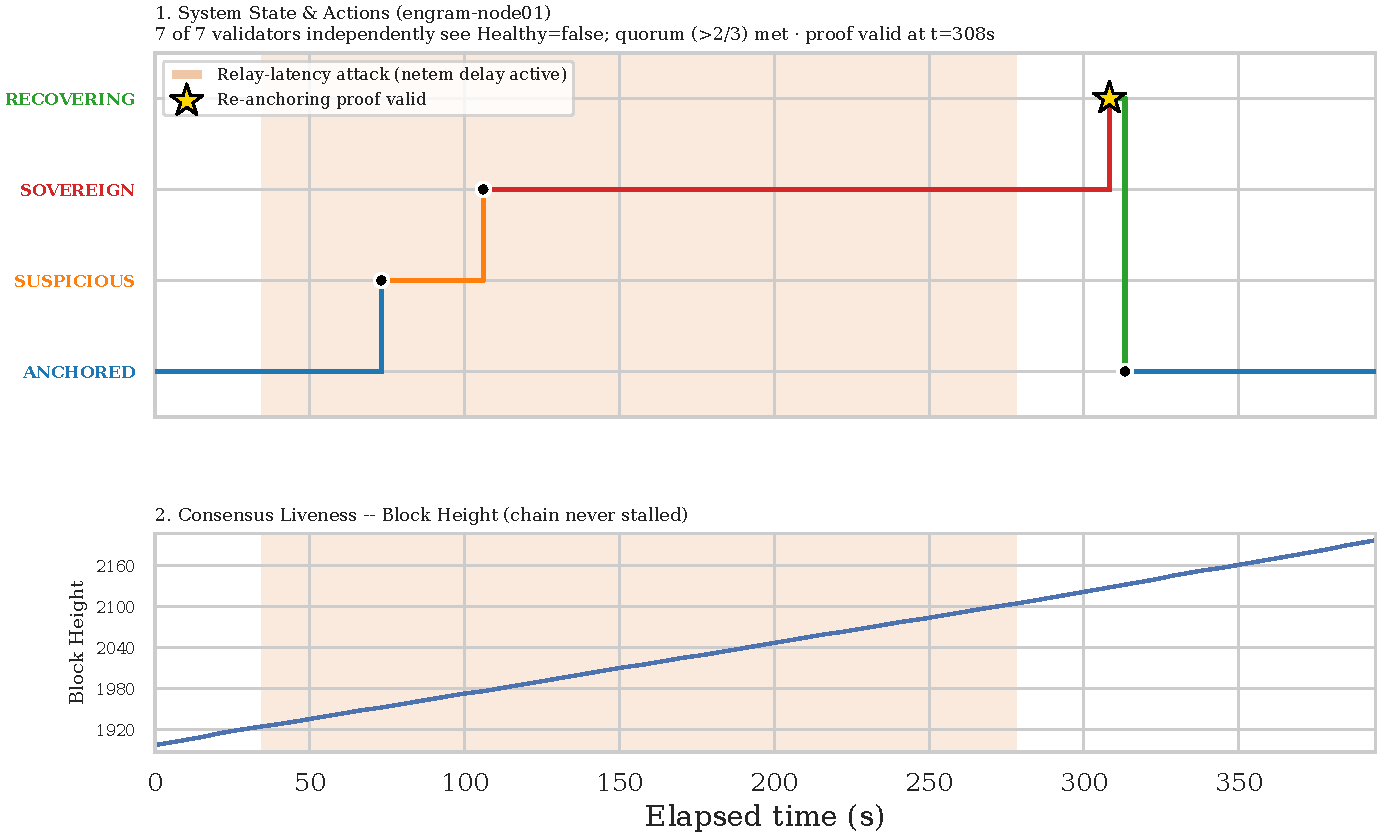
\includegraphics[width=\linewidth]{figures/p4_relay_cascade_timeline.pdf}
\caption{FSM cascade under a real, quorum-visible P2P relay-latency attack
(P4): all 7 validators independently sense the degradation, the transition
commits once quorum is met, and block production (bottom panel) never
stalls through the cascade or the recovery. An earlier single trial, with the heuristic fallback enabled; the three runs of the text used proof-only recovery.}
\label{fig:a4-cascade}
\end{figure}

P3 and P4 are two outcomes of one mechanism. The same kind of
sensor-confirmed degradation is ignored when a minority observes it and
drives a bounded cascade when all validators do, as Lemma~\ref{lem:honest-range} predicts: a
minority cannot move the certified aggregate, whereas a degradation seen by
every honest validator must move it.



\subsection*{Liveness and recovery: seven-scenario sweep, data availability and the adaptive threshold}

\textbf{Seven-scenario sweep.} The composite trace does not isolate which
failure mode drives which behavior. A second run therefore walks the chain
through seven sequential scenarios (Table~\ref{tab:schedule}): S1 healthy
baseline, S2 Bitcoin congestion (checkpoint submission suspended), S3 DA
outage (bridges stopped), S4 partial P2P eclipse, S5
anchor-peer isolation of one validator, S6 combined Bitcoin and DA failure,
and S7 recovery. Each scenario starts from the state the previous one left, and the
chain is given up to 600\,s to return to \textsc{Anchored} after S2--S5 and up to 900\,s in S7, with the heuristic fallback enabled. We ran the sequence seven
times, each on a freshly deployed chain (Fig.~\ref{fig:s1-s7} shows the first run).

\begin{figure}[tbp]
\centering
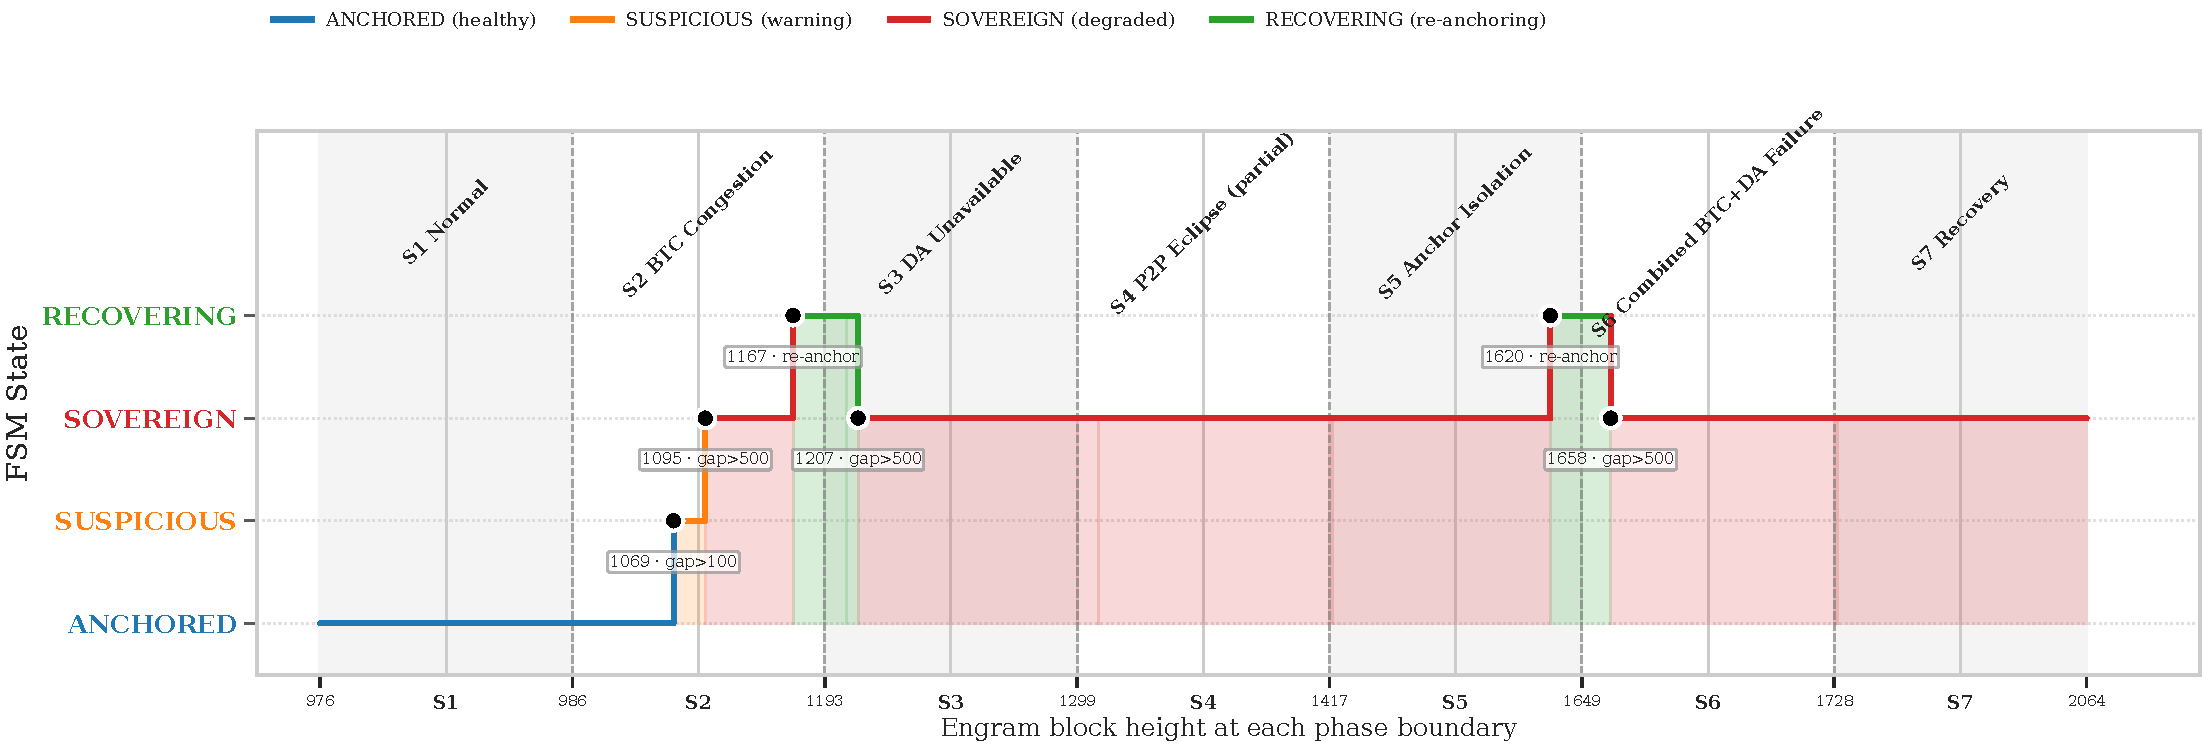
\includegraphics[width=0.95\linewidth]{figures/seven_scenario_timeline.pdf}
\caption{Continuous FSM-state timeline across seven sequential
fault-injection scenarios (S1--S7), true block-height ranges, live
7-validator testbed. Each scenario begins where the previous scenario's
recovery ended. Dots mark state changes; the lower axis gives the block height at each
phase boundary, and every phase has the same width. First of seven runs, heuristic fallback enabled.}
\label{fig:s1-s7}
\end{figure}

The chain kept committing blocks in every scenario of every run. S2 and S3
escalated through \textsc{Suspicious} to \textsc{Sovereign} in all seven runs: S2
after 143.5\,s on average (95\% interval $\pm$6.3\,s, Student $t$, range 133.8--153.3\,s)
and S3 after 30.5\,s ($\pm$1.6\,s, range 27.5--33.5\,s). S4 reached \textsc{Sovereign}
in all seven runs, after 72.8--110.7\,s in the six runs that entered it from \textsc{Anchored}.
S5 produced only a transient \textsc{Suspicious} excursion absorbed by hysteresis in all
six runs that entered it from \textsc{Anchored}: isolating one of seven validators from its anchor
peers leaves the certified active-anchor-peer count above zero, so the critical condition never
holds. S4 and S5 are therefore distinct failure classes rather than two intensities of one
signal. S6 entered \textsc{Sovereign} in every run.

The return to \textsc{Anchored} after S7 is where the runs differ. The chain entered
\textsc{Recovering} 16.6--19.6\,s after the faults were removed in six runs and then fell
back from \textsc{Recovering} to \textsc{Sovereign} between one and six times before
returning to \textsc{Anchored} at all seven validators. From entering \textsc{Recovering} to that return it took
331, 332, 334, 334 and 347\,s in five runs and 645\,s in the sixth, the run with six
fall-backs (median 334\,s; mean 387\,s with a 95\% interval of $\pm$133\,s, which the one long run dominates).
The seventh run did not return: after S4 it stayed in \textsc{Sovereign} through
S5, S6 and the 898\,s of S7, with all seven validators agreeing on it and the chain still
committing blocks (Section~\ref{subsec:limitations}). The statement that the chain returns to \textsc{Anchored}
after the faults are removed therefore holds in six of the seven runs, and the recovery time
is long and variable under the heuristic fallback.


\textbf{Data availability of the \textsc{Sovereign} interval.} The exit
condition of Section~\ref{subsec:reanchoring} requires the interval's block
data to be republished before \textsc{Recovering}$\to$\textsc{Anchored}. We
stopped all seven Celestia bridges for 120, 300 and 600\,s, restarted them, and
after the chain returned to \textsc{Anchored} re-fetched every height of the
interval from Celestia through \texttt{blob.GetAll}, comparing the bytes with
the Engram block. Table~\ref{tab:backfill} shows that all 2{,}291 heights over
nine runs were found and identical. The chain entered \textsc{Sovereign}
46--49\,s after the bridges stopped, and the time in \textsc{Recovering} did
not grow with the interval: 37--61\,s for 75--77 blocks and 49--61\,s for
465--475 blocks. The check is external to the chain: the gate itself rests on the
quorum-reported contiguous height, and these runs show that height was truthful
when all validators were honest. They cover a total DA outage on one host
with three runs per length. All runs use one bridge blob limit; the 600\,s outage is reported only at that limit, since the bridges did not survive it at 512\,MiB.
These runs kept the heuristic fallback of Section~\ref{subsec:reanchoring}
enabled (proof-only recovery off), so the time in \textsc{Recovering} does not
isolate the cost of the recovery proof; the data-availability results are
independent of that choice.
A gate that always opens would pass the runs above, so we also withheld
data. A test hook makes a validator publish only head markers: its DA liveness
stays healthy, so the chain can reach \textsc{Recovering}, but its contiguous
height never advances. The certified height is a weighted median over the
certificates, so the gate should hold when four or more of the seven
validators withhold data and open when three or fewer do. Table~\ref{tab:backfill-controls}
shows that it did in all seven runs. In a third control, two validators signed
a contiguous height of $10^{12}$ while the five honest ones withheld data; the
median stayed at zero and the gate held, as it should against $f{=}2$
misreporting validators. These controls use two to three runs per setting, each
on a freshly deployed cluster, and the withholding validators are a test
configuration, not a modelled adversary. The reported third control ran with all five withholding validators.

\begin{table}[tbp]
\caption{Republication of the \textsc{Sovereign} interval after a total DA
outage (three runs per outage length; range over runs; heuristic fallback enabled)}
\label{tab:backfill}
\centering
\footnotesize
\begin{tabular}{@{}rrrr@{}}
\toprule
\textbf{Outage (s)} & \textbf{Interval (blocks)} & \textbf{Time in \textsc{Recovering} (s)} & \textbf{Heights found, identical} \\
\midrule
120 & 75--77 & 36.6--61.1 & 229 / 229 \\
300 & 217--219 & 60.9--67.3 & 655 / 655 \\
600 & 465--475 & 49.0--61.2 & 1407 / 1407 \\
\bottomrule
\end{tabular}
\end{table}

\begin{table}[tbp]
\caption{Backfill-gate controls after a 120\,s DA outage (validators withholding
block data; the gate must hold for 300\,s or open; heuristic fallback enabled)}
\label{tab:backfill-controls}
\centering
\footnotesize
\begin{tabular}{@{}lrr>{\raggedright\arraybackslash}p{0.38\linewidth}@{}}
\toprule
\textbf{Setting} & \textbf{Runs} & \textbf{Interval (blocks)} & \textbf{Outcome} \\
\midrule
4 of 7 withhold data & 3 & 201--208 & held in \textsc{Recovering} 3 / 3 \\
3 of 7 withhold data & 2 & 67--72 & left \textsc{Recovering} after 34 and 43\,s; data identical \\
2 inflated claims + 5 withhold & 2 & 202--208 & held in \textsc{Recovering} 2 / 2 \\
\bottomrule
\end{tabular}
\end{table}

\textbf{Exploratory extension: an adaptive down threshold.} We also evaluated an
extension that raises $k_{\downarrow}$ after each flap and lowers it after
$T_{\text{stable}}$ healthy blocks (Section~\ref{subsec:transitions}). The result is
negative: in live runs it did not outperform a static threshold of 4 (no flap at a
detection delay of 13.7\,s), and its absorption of repeated short pulses rests on
simulation alone (Appendix~\ref{app:adaptive}). We therefore recommend a static
threshold of 4 or more (Section~\ref{sec:discussion}) and treat the backoff as an
extension, not a contribution.

Appendix~\ref{app:reorg} complements these results by measuring how deep a
real Bitcoin reorganization must be before the FSM reacts.



\subsection*{Cost: certificate scaling and load sensitivity}

\textbf{Where the cost is not.} Each proposal carries the health certificate as
its first transaction: one signed vote extension per validator in the quorum plus
the leader's claimed aggregation. At seven validators it is \resProposalBytes\,bytes on
average (live, ANCHORED; 889--926 across states, 300 consecutive blocks), which
splits into a fixed 70\,bytes and 118 per validator (22 for the address, 28 for
the extension, 66 for the signature). The signatures are a copy of the vote
extensions, kept in the proposal because \texttt{ProcessProposal} receives none
under ABCI~2.0; they are separate from the signatures in the block's last commit,
so the cost is paid twice. The one proof-carrying
block observed was 14.9\,KB, consistent with the 14.7\,KB proof.
Validating an accepted proposal, including the ed25519 verification of one
signature per validator, costs \resValidationUs\,$\mu$s per block at seven
validators (mean of ten benchmark runs on the final commit with the machine idle, standard deviation 13\,$\mu$s).
Size and
validation time are linear in the number of validators
(Table~\ref{tab:cert-scaling}); we measured the block interval only at seven
validators, so the larger rows are a microbenchmark of the certificate, not a
measurement of a larger network. Verifying a recovery proof, a one-off event,
takes 26\,ms and is not included. \texttt{ExtendVote}, which reads the live
Bitcoin and Celestia sensors before a validator can precommit, takes
\resExtendVoteMs\,ms on average (p95 51\,ms, five repeats) and does not depend on
the number of validators, since each validator reads only its own sensors. None
of these is large enough to explain a lower block rate at a $\sim$1\,s block
interval at seven validators.

\begin{table}[tbp]
\caption{Certificate size and \texttt{ProcessProposal} time against the number of
validators (microbenchmark of the shipped code with real ed25519 signatures, one
core, ten runs; sizes are from the benchmark fixture, whose extensions are about
15\% smaller than the live ones, so the live size at $n{=}7$ is 894 against 776\,bytes).}
\label{tab:cert-scaling}
\centering
\footnotesize
\begin{tabular}{@{}rrr@{}}
\toprule
\textbf{Validators} & \textbf{Certificate, bytes} & \textbf{\texttt{ProcessProposal}, $\mu$s (sd)} \\
\midrule
4 & 473 & 181 (7) \\
7 & 776 & 301 (13) \\
16 & 1{,}685 & 638 (21) \\
32 & 3{,}301 & 1{,}242 (22) \\
64 & 6{,}533 & 2{,}466 (58) \\
\bottomrule
\end{tabular}
\end{table}

\textbf{Where the cost is.} Against a single local process, Engram's blocks
arrive 0.23\,s later (\resBlockEngram{} against 1.034\,s). Table~\ref{tab:overhead} shows
that this gap is not Engram's. Seven vanilla validators on the same hosts,
network, genesis and load produce a block every \resBlockVanilla\,s with vote extensions
disabled and every 1.229\,s with empty extensions, within 0.03\,s of Engram
(95\% CIs of 0.015--0.023\,s). Hence the 0.2\,s is the price of running a
seven-validator BFT network on one host, and vote extensions as such add no
measurable time. The paired design isolates Engram's own addition. It alternates the two arms on
fresh deployments of the same hosts, genesis and load, with the arm that runs first
alternating, so that drift of the host cancels within a pair. Over 20 pairs Engram's
block interval exceeds the vanilla one by 0.022\,s per height (1.8\%;
\resPairedEngram\,s against \resPairedVanilla\,s). The 95\% interval is 0.005 to
0.038\,s from the Student $t$ distribution on the pair differences and 0.008 to
0.038\,s from a bootstrap over pairs; it excludes zero, so Engram adds a small cost,
of the order of the \resExtendVoteMs\,ms \texttt{ExtendVote} time. One pair
(+0.144\,s) is an outlier; without it the estimate is 0.015\,s (0.005 to 0.026\,s).
We planned to stop when the half-width fell below 0.012\,s or at 20 pairs; at 20 pairs
it was 0.017\,s, so the interval is wider than planned. The unpaired deployments of
Table~\ref{tab:overhead} agree: the three Engram deployments average 1.2707, 1.2423 and
1.2620\,s and the two seven-validator vanilla deployments 1.2292 and 1.2331\,s, a
difference of 0.027\,s with a 95\% interval of $-$0.008 to 0.062\,s from the pooled
between-deployment spread (0.012\,s, three degrees of freedom). The repeats of one
arm share a chain, so the unit of independence is the deployment. Those arms ran on
separate deployments except the first Engram and the extensions-on arm, which shared
one chain (Engram first); the Engram arm was repeated on a fresh deployment to check
for an order effect and moved by 0.02\,s.


\textbf{Load sensitivity.} Table~\ref{tab:overhead} is measured at 20\,tx/s. Both
systems accepted every submitted transaction into the mempool across an
earlier 5--100\,tx/s ramp, but mempool acceptance is not throughput. To see how
the two systems respond to load we offered 20, 50, 100, 200 and 500\,tx/s for
60\,s with five repeats per rate and drained the mempool after each
(Table~\ref{tab:throughput}). We did not look for a throughput ceiling, which one
host cannot give: vanilla CometBFT and Engram committed every offered
transaction at every rate, so neither saturated, and the limit we hit first was
CPU, with the busiest validator at 64--83\% at 500\,tx/s on a host that runs all
seven. What separates the systems is latency: the p95 stays at 1.5--1.9\,s for
vanilla, while Engram's rises from 2.2\,s at 100\,tx/s to 6.5\,s at 500\,tx/s.

\begin{table}[tbp]
\caption{Load sensitivity under open-loop offered load, seven validators on one host (60\,s per repeat,
five repeats; mean $\pm$ 95\% Student-$t$ interval). The \textsc{Anchored}
share is the fraction of two-second samples of one validator's FSM state spent
in \textsc{Anchored} and was recorded for the third arm only.}
\label{tab:throughput}
\centering
\footnotesize
\resizebox{\linewidth}{!}{\begin{tabular}{@{}rlrrrr@{}}
\toprule
\textbf{Offered (tx/s)} & \textbf{Arm} & \textbf{Committed (tx/s)} & \textbf{p95 latency (s)} & \textbf{Peak CPU (\%)} & \textbf{\textsc{Anchored} share} \\
\midrule
20 & Engram & 20 $\pm$ 0 & 1.6 $\pm$ 0.1 & 10 $\pm$ 2 & -- \\
20 & Vanilla & 20 $\pm$ 0 & 1.6 $\pm$ 0.1 & 8 $\pm$ 3 & -- \\
\addlinespace
50 & Engram & 50 $\pm$ 0 & 1.7 $\pm$ 0.0 & 15 $\pm$ 8 & -- \\
50 & Vanilla & 50 $\pm$ 0 & 1.6 $\pm$ 0.0 & 12 $\pm$ 2 & -- \\
\addlinespace
100 & Engram & 100 $\pm$ 0 & 2.2 $\pm$ 0.4 & 29 $\pm$ 6 & -- \\
100 & Engram, peer-latency bound 5000\,ms & 100 $\pm$ 0 & 1.7 $\pm$ 0.1 & 21 $\pm$ 5 & 0.83 $\pm$ 0.09 \\
100 & Vanilla & 100 $\pm$ 0 & 1.6 $\pm$ 0.1 & 19 $\pm$ 11 & -- \\
\addlinespace
200 & Engram & 200 $\pm$ 0 & 3.8 $\pm$ 0.8 & 81 $\pm$ 11 & -- \\
200 & Engram, peer-latency bound 5000\,ms & 200 $\pm$ 0 & 1.9 $\pm$ 0.5 & 39 $\pm$ 23 & 0.13 $\pm$ 0.37 \\
200 & Vanilla & 200 $\pm$ 0 & 1.5 $\pm$ 0.1 & 23 $\pm$ 5 & -- \\
\addlinespace
500 & Engram & 500 $\pm$ 0 & 6.5 $\pm$ 0.8 & 83 $\pm$ 12 & -- \\
500 & Engram, peer-latency bound 5000\,ms & 500 $\pm$ 0 & 4.6 $\pm$ 1.1 & 73 $\pm$ 11 & 0.00 $\pm$ 0.00 \\
500 & Vanilla & 500 $\pm$ 0 & 1.9 $\pm$ 0.4 & 64 $\pm$ 30 & -- \\
\addlinespace
\bottomrule
\end{tabular}
}
\end{table}

At 20\,tx/s the addition of Engram is a few percent of the block
interval (Table~\ref{tab:overhead}); as the load grows, latency grows and the FSM
leaves \textsc{Anchored} for part of the time, already at 100\,tx/s, as follows. The
Engram figures from 100\,tx/s upward are not a steady \textsc{Anchored}
state. The peer-latency sensor read round-trip times of up to 1.2\,s between
validators under this load in the first Engram arm, above the 200\,ms bound, so we repeated the sweep
with the bound raised to 5000\,ms. The chain still left \textsc{Anchored}:
the share was 0.83 at 100\,tx/s, 0.13 at 200\,tx/s and 0 at 500\,tx/s, so the
peer-latency bound is not the only reason. A second candidate is the DA
check: under load its RPC may exceed its timeout and read as a failed layer. We
repeated the runs at 200 and 500\,tx/s on fresh deployments, three each, with the
DA RPC timeout raised to 90\,s and the DA check timeout to 2.5\,s, against three
runs with the defaults. The share of samples in \textsc{Anchored} rose from 0.68 to
0.75 at 200\,tx/s and from 0.36 to 0.80 at 500\,tx/s, where the default runs also
reached \textsc{Sovereign} and the relaxed ones did not; the relaxed runs still
left \textsc{Anchored}, so the DA timeouts explain part of the departure and not
all of it. In the relaxed runs at 500\,tx/s the p95 latency was 3.1--4.6\,s and the
peak validator CPU was 42--46\% (three runs).
That arm had lower latency than the default one (p95 1.9 against 3.8\,s at
200\,tx/s) and was still above vanilla. We therefore cannot separate the cost of
the consensus extension from the effect of a demoted FSM above 100\,tx/s on
this host, and report only that Engram's latency grows with load where
vanilla's does not. All seven validators share the host's cores, so absolute
values do not transfer to separate machines, and one host does not support a
claim about production throughput or scalability. The 5000\,ms bound was set
through the environment of that deployment, whose genesis we did not keep; the
first Engram arm did not record the FSM state.



\subsection*{Discussion: additional security analyses and the testbed gap}

\textbf{Repeated triggering of \textsc{Suspicious}.} An adversary that repeatedly
pushes the chain into \textsc{Suspicious} is limited only by the bounded
forced-transaction queue and the down threshold. An optional backoff of the down
threshold, which we did not evaluate on the \textsc{Recovering}$\to$\textsc{Sovereign}
edge, was meant to raise the price of such repetition. On the
\textsc{Anchored}$\to$\textsc{Suspicious} edge it did not beat a static threshold of 4
in live runs, and its absorption of short pulses has no live evidence
(Appendix~\ref{app:adaptive}).


\textbf{Hysteresis: noise against concealment.} A higher down threshold $k$
tolerates longer bursts of noise, and it also tolerates a longer run of reports
that a Byzantine proposer interleaves with honest ones. Within the assumption the
choice of $k$ does not matter for detection: for each of the 21 placements of two
Byzantine proposers in the seven-slot rotation, a real DA outage was detected after
exactly $k$ blocks ($k\in\{2,3,4\}$, simulation). With three Byzantine validators,
outside the assumption, a larger $k$ makes concealment easier: in the simulation
the outage was missed for 14 of 35 placements at $k{=}3$ and for 28 at $k{=}4$. The
live runs at $k{=}2$ detected it in 5 of 5 runs; at $k{=}4$ the live runs did not
reproduce the simulation's concealment for interleaved placements, so concealment
at $k{=}4$ rests on the simulation alone. The experiments ran with
$k_{\downarrow}{=}2$, which the live noise sweeps show to be too low for a
wide-area network (flapping, 82\% of the noisy phase in \textsc{Anchored}); we
recommend $k_{\downarrow} \geq 4$ as a deployment setting, set from the noise of
the environment, at the price of easier concealment. Appendix~\ref{app:envelope}
gives the detail, including a window rule that is not cut by interleaving and that
we did not implement.


\textbf{Testbed gap.} Four properties of the testbed limit how its results transfer to a
production deployment.
\begin{itemize}
  \item \emph{Single physical host.} All Testbed~A containers share one
  machine's CPU and memory, so resource contention can affect every validator
  at once; wide-area conditions are emulated with \texttt{tc netem} rather
  than real geographic distribution.
  \iftestbedB Testbed~B removes both limitations for the experiments repeated
  on it (so far the proving-latency runs; its composite and load runs are
  pending).\fi
  \item \emph{Accelerated Bitcoin.} Regtest blocks arrive about $30\times$
  faster than on mainnet. Height-based thresholds are unaffected, but
  wall-clock durations scale accordingly.
  \item \emph{DA payload.} The DA publisher submits the transactions of
  committed blocks in height-ordered batches of at most 1.5\,MB and tracks
  the highest contiguous published height; the exit gate of
  Section~\ref{subsec:reanchoring} requires that height to cover the
  \textsc{Sovereign} interval. The gate rests on a quorum-reported
  contiguous height, not on a cryptographic proof of retrievability.
  Section~\ref{subsec:rq3} reports the republication of the interval after a
  live DA outage.
  \item \emph{Single-bridge trust.} Each validator trusts its own bridge
  node, which downloads and verifies full Celestia blocks, rather than
  sampling across independent peers; our DA-outage results measure bridge
  failures, not sampling-detected partial withholding.
\end{itemize}



\subsection*{Protocol: sensor definitions and long intervals}

\textbf{Bitcoin finality gap.} $\Delta H_{\text{BTC}} = H_{\text{current}} -
\min(H_{\text{submitted}}, H_{\text{anchored}})$ measures how far the latest
checkpoint lags Bitcoin's tip; it grows under congestion or checkpoint
censorship. Because a delay metric cannot detect a checkpoint that was
reorganized away, each validator also re-verifies, against its own Bitcoin
full node, that the checkpoint transaction is still included at depth
$\geq K_{\text{DEEP\_FINALITY}}$. A failed re-verification is a critical
condition.

\textbf{DA gap.} $\Delta H_{\text{DA}} = H_{\text{local}} -
H_{\text{verified}}$ measures the lag between the chain head and the highest
height whose DA submission the validator has confirmed as retrievable from
its own Celestia bridge node. This is bridge-level retrievability, not a
data-availability-sampling proof; Section~\ref{subsec:sim-to-real} describes
what the prototype publishes.

\textbf{Units of the gaps.} The two gaps count different things because the two
layers guarantee different things. The Bitcoin gap counts Bitcoin blocks, since a
checkpoint's guarantee is its confirmation depth; it grows only with the Bitcoin
blocks that arrive while no checkpoint is anchored, so a slow Bitcoin chain adds no
gap. The DA gap counts Engram heights, since the guarantee of the DA layer is that
every Engram height is retrievable. Each threshold is read in the unit of its own
layer and converts to time at that layer's cadence: a Bitcoin block takes 600\,s on
mainnet and 20\,s on the testbed, an Engram block about 1.2\,s on both. A time bound
that must cover a Bitcoin fault, such as the \textsc{Suspicious} timeout
$T_{\text{sus}}$ (Section~\ref{subsec:transitions}), therefore follows the Bitcoin
cadence of the deployment (Section~\ref{sec:discussion}).

\textbf{P2P health.} Peer count alone cannot distinguish a long-lived honest
peer from a fresh Sybil, and eclipse attacks combine vectors no single
metric captures~\cite{rehman2025eclipse,heilman2015eclipse}. The profiler
combines six bounds -- subnet diversity, active anchor peers, clean peers,
churn rate, mean peer tenure, and latency -- applied to the Engram P2P
interface, the Bitcoin client, and the Celestia client. These bounds
characterize peripheral and partial P2P degradation; a partition of the
core consensus network below a quorum is outside what any FSM can handle
(Section~\ref{sec:intro}).


\textbf{Longer intervals.} An interval longer than 256 headers is covered by
a sequence of proofs: each accepted proof advances the on-chain
$\mathit{rt}_{\text{last}}$ to its $\mathit{rt}_{\text{new}}$, and the next
proof must start from that root. This costs $\lceil L/256 \rceil$ proofs for
$L$ blocks. An aggregator circuit can fold up to four chunk proofs into one
proof of the same size, which makes verification cost independent of $L$ up to
1024 headers at the price of one extra proof; proving time still grows with $L$
(Table~\ref{tab:recovery-cost}, Appendix~\ref{app:aggregation}).

\begin{table}[tbp]
\caption{Cost of the recovery proof by interval length $L$ (offline workstation,
synthetic chain; one by one against aggregate, from Appendix~\ref{app:aggregation})}
\label{tab:recovery-cost}
\centering
\footnotesize
\begin{tabular}{@{}rlrrr@{}}
\toprule
$L$ & Submission & Prove & Bytes & Verify \\
\midrule
256 & single proof & 31.5\,s & 14{,}656 & 19.8\,ms \\
512 & aggregate of 2 & 89.9\,s & 14{,}656 & 20.2\,ms \\
512 & one by one & 60.5\,s & 29{,}312 & 39.5\,ms \\
1024 & aggregate of 4 & 146.7\,s & 14{,}656 & 20.2\,ms \\
1024 & one by one & 120.1\,s & 58{,}624 & 79.1\,ms \\
\bottomrule
\end{tabular}
\\[2pt]
\footnotesize Verify is the validators' embedded WebAssembly verifier, per proof (30
iterations, three runs); the one-by-one rows are $n$ times the leaf cost, and the
aggregate's proving time includes its leaf proofs. Aggregate proving and verification
are averaged over five trials per length, each leaf proof was timed once, and the chain
is synthetic (Appendix~\ref{app:aggregation}).
\end{table}

The aggregate has a constant size and verification time, and costs more to prove than
the chunks alone; the prover's chunks were built one after another, and proving them
concurrently was not measured.



\subsection*{Related-work taxonomy and fault schedules}

\begin{figure}[p]
\centering
\begin{tikzpicture}[
  font=\scriptsize, >=Stealth,
  box/.style={draw, rounded corners, inner sep=2.5pt, align=left, anchor=west},
  root/.style={box, fill=gray!12, text width=2.1cm},
  q/.style={box, text width=3.2cm, minimum height=0.6cm},
  leaf/.style={box, text width=8.2cm, minimum height=0.6cm},
  hl/.style={fill=blue!8}]
\node[leaf] (l1) at (6.9,-0.00) {Fast path with fallback; protocol switching on internal faults~\cite{pass2018thunderella,aublin2015next700,giridharan2024autobahn}};
\node[leaf] (l2) at (6.9,-0.95) {Availability--finality trade-offs on internal participation~\cite{pass2017sleepy,neu2021ebbflow,buterin2017casper,buterin2020gasper}};
\node[leaf, hl] (l3) at (6.9,-1.90) {\textbf{Degradation triggered by the health of external layers (Engram)}};
\node[q] (q0) at (3.1,-0.95) {Q1. How does consensus behave under degraded conditions?};
\draw[->] (q0.east) -- ++(0.25,0) |- (l1.west);
\draw[->] (q0.east) -- ++(0.25,0) |- (l2.west);
\draw[->] (q0.east) -- ++(0.25,0) |- (l3.west);
\node[leaf] (l4) at (6.9,-3.05) {Local failure detectors, including Byzantine muteness~\cite{chandra1996unreliable,chen2002qos,hayashibara2004phi,doudou1999muteness}};
\node[leaf] (l5) at (6.9,-4.00) {Aggregation of Byzantine inputs~\cite{dolev1986approximate,stolz2015median}};
\node[leaf] (l6) at (6.9,-4.95) {Blockchain oracles~\cite{zhang2016towncrier,eskandari2021oraclesok,xiao2023decentruth,yao2025pscbo}};
\node[leaf] (l6b) at (6.9,-5.90) {Signed external data in vote extensions~\cite{cosmos_adr064,slinky_oracle}};
\node[leaf, hl] (l7) at (6.9,-6.85) {\textbf{Quorum-backed external-layer health as a control input to consensus (Engram)}};
\node[q] (q1) at (3.1,-4.95) {Q2. How do local observations of an external layer become consensus-visible data?};
\draw[->] (q1.east) -- ++(0.25,0) |- (l4.west);
\draw[->] (q1.east) -- ++(0.25,0) |- (l5.west);
\draw[->] (q1.east) -- ++(0.25,0) |- (l6.west);
\draw[->] (q1.east) -- ++(0.25,0) |- (l6b.west);
\draw[->] (q1.east) -- ++(0.25,0) |- (l7.west);
\node[leaf] (l8) at (6.9,-8.00) {DA layers and fraud proofs~\cite{albassam2019lazyledger,albassam2021fraud,phamminh2026cda}};
\node[leaf] (l9) at (6.9,-8.95) {Bitcoin checkpointing~\cite{karakostas2021checkpointing,tas2022babylon,azouvi2022pikachu,tas2023bitcoinpos}};
\node[leaf] (l10) at (6.9,-9.90) {Rollup fallback: escape hatch, DA-committee fallback, Alt-DA challenges, decentralized sequencers~\cite{figueira2025escapehatch,arbitrum_anytrust,optimism_altda,capretto2025secure,capretto2026setconsensus}};
\node[leaf, hl] (l11) at (6.9,-10.85) {\textbf{Validity rules and withdrawals switched by quorum-backed health (Engram)}};
\node[q] (q2) at (3.1,-9.40) {Q3. How do modular designs cope with failure of Bitcoin, DA, or settlement layers?};
\draw[->] (q2.east) -- ++(0.25,0) |- (l8.west);
\draw[->] (q2.east) -- ++(0.25,0) |- (l9.west);
\draw[->] (q2.east) -- ++(0.25,0) |- (l10.west);
\draw[->] (q2.east) -- ++(0.25,0) |- (l11.west);
\node[leaf] (l12) at (6.9,-12.00) {Succinct header-chain proofs and light clients~\cite{xie2022zkbridge,vesely2022plumo,bonneau2020mina,bunz2020flyclient}};
\node[leaf] (l13) at (6.9,-12.95) {Recursion and folding~\cite{bitansky2013recursive,bowe2019halo,kothapalli2022nova}};
\node[leaf, hl] (l14) at (6.9,-13.90) {\textbf{Chunked proof of interval continuity, mode and lock labels, and boundary quorum (Engram)}};
\node[q] (q3) at (3.1,-12.95) {Q4. How does a chain return to the anchored state?};
\draw[->] (q3.east) -- ++(0.25,0) |- (l12.west);
\draw[->] (q3.east) -- ++(0.25,0) |- (l13.west);
\draw[->] (q3.east) -- ++(0.25,0) |- (l14.west);
\node[leaf] (l15) at (6.9,-15.05) {Model checking and deductive proof~\cite{konnov2019apalache,braithwaite2020tendermint,padon2016ivy,hawblitzel2015ironfleet,wilcox2015verdi,qiu2024lido}};
\node[leaf] (l16) at (6.9,-16.00) {Fault injection~\cite{bano2021twins,basiri2016chaos}};
\node[leaf, hl] (l17) at (6.9,-16.95) {\textbf{Layered model checking plus live fault injection against Bitcoin and Celestia (Engram)}};
\node[q] (q4) at (3.1,-16.00) {Q5. How are such designs validated?};
\draw[->] (q4.east) -- ++(0.25,0) |- (l15.west);
\draw[->] (q4.east) -- ++(0.25,0) |- (l16.west);
\draw[->] (q4.east) -- ++(0.25,0) |- (l17.west);
\node[root] (r) at (0,-8.45) {A chain whose validity depends on external layers};
\draw[->] (r.east) -- ++(0.25,0) |- (q0.west);
\draw[->] (r.east) -- ++(0.25,0) |- (q1.west);
\draw[->] (r.east) -- ++(0.25,0) |- (q2.west);
\draw[->] (r.east) -- ++(0.25,0) |- (q3.west);
\draw[->] (r.east) -- ++(0.25,0) |- (q4.west);
\end{tikzpicture}
\caption{Taxonomy of related work, organized by the question each line of work
answers. Shaded leaves mark where Engram sits. Vote-extension oracles supply
signed external data to consensus (Q2) but attach no fallback semantics to it.}
\label{fig:taxonomy}
\end{figure}


\label{subsec:schedules}

Network-level faults use kernel traffic control (\texttt{tc netem} via
Pumba): uniform delay and jitter, packet loss, single-node isolation, and a
heterogeneous per-validator wide-area profile approximating seven regions.
Appendix~\ref{app:netem} lists the parameters of every profile. The
\emph{WAN latency baseline} is the per-validator delay and jitter profile of
Table~\ref{tab:netem-wan}, held for the whole run unless a step in
Table~\ref{tab:schedule} suspends it.

Application-level faults reproduce mechanisms that delay alone cannot, and
each simulates the consequence of a failure rather than its cause.
\begin{itemize}
  \item \emph{Bitcoin congestion} suspends the submission of new
  checkpoints (a pending one still confirms), so the finality gap grows
  directly. It does not congest the Bitcoin mempool.
  \item \emph{DA outage} stops one or all seven Celestia bridge containers.
  It does not emulate a data-availability-sampling failure.
  \item \emph{Byzantine behavior} is injected through attacker processes or
  through a validator configured to forge proposal fields, omit
  transactions, double-sign, or flood timeout messages.
\end{itemize}
Every fault targets a peripheral layer or a minority of validators; none
partitions the core consensus network below a quorum, consistent with the
scope defined in Section~\ref{sec:intro}.


Table~\ref{tab:schedule} gives the onset, mechanism, and duration of each
fault in the two scripted runs of Section~\ref{subsec:rq2}. Times are
relative to the start of each run, durations are the length of the polling
window the script holds the fault for, and each of S2--S5 is followed by a
wait of up to 600\,s for the validators to return to \textsc{Anchored} before
the next scenario starts.

The table is in Appendix~\ref{app:setup}: the composite run holds a Bitcoin fault, adds a DA outage, cycles packet loss on two validators, heals, and waits for recovery; the seven-scenario sweep applies one fault at a time (S2--S6) between a healthy baseline and a recovery wait.

\subsection*{Related work: failure detectors, aggregation, oracles, vote extensions and validation}

\textbf{Failure detectors.}
Unreliable failure detectors~\cite{chandra1996unreliable}, their QoS
metrics~\cite{chen2002qos}, and accrual detectors~\cite{hayashibara2004phi}
give each process a local, eventually accurate suspicion of other processes.
Muteness failure detectors~\cite{doudou1999muteness} extend the abstraction to
Byzantine processes that stop sending the messages an algorithm expects while
possibly continuing to send others. Engram's
sensors play the same role for peripheral layers, with two differences:
a local suspicion has no effect until a quorum of signed observations backs it, and the adversary
controls up to $f$ of the reporters.

\textbf{Aggregating Byzantine observations.}
Approximate agreement~\cite{dolev1986approximate} requires non-faulty
processes to decide on values that are close together rather than identical.
Median validity~\cite{stolz2015median} requires the decision to be close to the
median of the non-Byzantine inputs and, at maximal fault tolerance with
$n \geq 3t+1$, within the range of those inputs. The Engram health
certificate satisfies an analogous range-validity property for each
weighted-median metric. It does not run a second approximate-agreement
protocol: validators sign individual height-bound sensor snapshots carried as
vote extensions, CometBFT agrees on the proposal that carries them, and every
validator then recomputes the aggregate deterministically
(Section~\ref{subsec:health-certificate}).

\textbf{Blockchain oracles.}
Oracle research addresses how replicated applications import external
information. Town Crier authenticates web data with trusted
hardware~\cite{zhang2016towncrier}. A systematization of oracle designs
classifies their trust assumptions and manipulation
risks~\cite{eskandari2021oraclesok}. DecenTruth combines multi-source truth
discovery with decentralized consensus to tolerate dishonest
reports~\cite{xiao2023decentruth}, and PSCBO analyzes attacks on consensus-based
oracle designs~\cite{yao2025pscbo}. In all of these, the oracle supplies a value
to the application layer.

\textbf{Vote extensions.}
The closest mechanism to Engram's certificate is the ABCI++ vote extension.
Each validator extends its precommit with application data, which may be
obtained non-deterministically, and the next proposer includes the signed
extensions in its proposal. The Cosmos SDK design record requires signatures
from at least two thirds of the voting power and uses an oracle price fetcher
as its example~\cite{cosmos_adr064}; Slinky applies the pattern to off-chain
price data and aggregates the extensions with a stake-weighted
median~\cite{slinky_oracle}. Engram uses the same transport: sensor snapshots
taken at height $H$ reach the proposer at $H{+}1$, where their deterministic
aggregation forms the health certificate. The difference lies in what the
aggregate controls. A price oracle supplies a value to the application; the
health certificate describes the infrastructure on which block validity
depends and determines the receipt requirements, the withdrawal policy, and
the entry into and exit from a degraded mode.

\textbf{Peripheral P2P attacks.}
Sybil attacks~\cite{douceur2002sybil}, in which one entity presents multiple
identities, and eclipse attacks on Bitcoin's P2P
layer~\cite{heilman2015eclipse,rehman2025eclipse}, which monopolize a node's
connections, let an adversary control what a node sees of an external network. They motivate the multi-signal peer-health
profile that Engram's P2P sensor uses and are one reason a single local reading
is not trusted.

\subsection{Validation Methodology}
\label{subsec:rw-validation}
TLA+~\cite{lamport2002specifying} with TLC and
Apalache~\cite{konnov2019apalache} has been used to specify and model-check
Tendermint's blockchain synchronization protocol~\cite{braithwaite2020tendermint}. Deductive approaches establish properties by machine-checked proof instead of
by exploring a bounded instance. Ivy~\cite{padon2016ivy} verifies safety of
infinite-state systems interactively, and Lotan and
Shoham~\cite{lotan2025implicit} automate liveness proofs in first-order logic
over finite but unbounded domains. IronFleet~\cite{hawblitzel2015ironfleet} and
Verdi~\cite{wilcox2015verdi} verify distributed-system implementations, the
latter in Coq, and LiDO~\cite{qiu2024lido} gives mechanized safety and
liveness proofs in Coq for unpipelined and pipelined Jolteon. A recent
preprint places these approaches on a maturity
scale~\cite{bondarev2026sok}. Engram sits in the model-checking family, with a
per-layer result and an open refinement obligation
(Section~\ref{sec:formal}). On the empirical side, Twins~\cite{bano2021twins}
tests BFT implementations by duplicating validator identities, and chaos
engineering~\cite{basiri2016chaos} injects faults into production systems.
Engram's evaluation combines network-level and application-level fault
injection against live Bitcoin and Celestia networks.


\subsection*{Protocol: lemma limits, certificate binding and the intended verifier}

\textbf{What the lemma does not give.} It bounds each metric separately. The
aggregate vector need not equal the observation of any honest validator, so a
condition on several metrics can hold of $\mathsf{Agg}(C^{h})$ when it holds of
no honest observation. For example, with three equally weighted honest
validators and three metrics, each validator seeing a different metric beyond
its threshold, every aggregated metric is within its threshold although every
honest validator sees a degradation. The lemma also does not say which honest
value the aggregate takes when honest values differ (see the proposer
discussion below).

\textbf{Adversarial cases.} The lemma does not require honest observations to
agree; it bounds what the adversary can do when they disagree, and each
adversarial case reduces to it (Appendix~\ref{app:certificate}). A stale or
replayed observation fails the height and round binding, two observations by one
validator count once, and false observations below $W/3$ cannot leave the honest
range. The proposer chooses the set $S$ and may omit honest observations; if $S$
still meets (d) the lemma holds, and if not, the certificate is not well-formed
and honest validators reject the proposal. The proposer's residual influence is
choosing \emph{which} honest value in the honest range is selected when honest
validators genuinely disagree: with $n{=}7$ equal-power validators and a quorum
of $q{=}5$ it reaches the third to the fifth smallest observation, the median of
all seven being the fourth. Only when honest observations straddle a threshold
does this choice change a decision, and a transition needs the hysteresis count
over consecutive blocks while proposers rotate, so a Byzantine proposer influences
the blocks it proposes. In the live collusion suite (Section~\ref{sec:evaluation},
case B3), honest validators accepted a proposer that kept exactly a quorum of
certificates in 3 of 3 repeats and rejected one that kept fewer, 210 times in total
across the 3 repeats.

\textbf{Height and round binding.} The certificate committed at height $h$
describes observations signed at height $h{-}1$, one block of lag. A
signature binds $(\mathit{chainID}, h{-}1, r, m_i)$, and a well-formed
certificate takes observations only from the commit round $r^{\star}$ and
only from validators whose precommit is in that commit.
This prevents replay of an observation from another height or round into
$C^{h}$. The binding is a property of the consensus instance, not of the
measurement: a validator can still sign a cached Bitcoin tip or stale peer
metrics (Section~\ref{subsec:sensors}).

\textbf{Intended verifier.} A CometBFT quorum certificate shows that a quorum
signed a block. The recovery proof adds a statement about the headers
that the chain recorded between two signed blocks: each records \textsc{Sovereign}
or \textsc{Recovering} with the lock flag set. The circuit does not tie the header
chain to the two signed blocks; the public inputs do, and a verifier must compare
them with its own record of the roots, the height of the first block and the hashes
of the two boundary blocks. This matters to a verifier that
does not replay the chain, such as a bridge or light client on another chain,
a node syncing from genesis, or a Bitcoin observer
(Section~\ref{subsec:security-semantics}). For validators, which already hold
the headers, it is a consistency check. The target verifier is an external
light client that accepts a re-anchoring checkpoint only with a valid proof;
the prototype does not include such a client.
As a check that the proof can be verified without the node, a separate
process on the same host read a committed block over RPC, took the proof (14{,}656\,bytes) and
the 224-byte public inputs from its recovery-proof transaction, and verified them
with \texttt{bb} against the verification key shipped with the repository; this was
one proof on one chain.

Intervals longer than 256 headers and the proving cost by length (Table~\ref{tab:recovery-cost}) are in Appendix~\ref{app:extended}.


\subsection*{Formal analysis: certificates in the model and the refinement}

\textbf{Health certificates in the model.} The server layer models each
validator's observation as three Booleans (healthy, warning, critical) and the
Bitcoin and DA gaps clipped to $0..3$; the aggregate is a per-field majority for
the Booleans and a weighted median for the gaps, and \texttt{IsValidProposal}
rejects a certificate below a quorum. A Byzantine validator may sign any
observation; an honest validator with an eclipsed P2P layer may report a degraded
one, never a healthier one, which is a sensor-soundness assumption of the model.
Every validator has the same voting power, and the proposer may choose any member
set that forms a quorum.

Lemma~\ref{lem:honest-range} is checked as \texttt{AggWithinHonestRange} with Apalache, with the
observation vector left symbolic so that one check covers every vector. For
$N{=}4$ and $f{=}1$ it reported no violation (22\,s). With two Byzantine
validators in the same network it reports a violation (25\,s), so the bound
on Byzantine members is necessary. Signatures, height and round binding,
and the individual P2P counters are not modelled. The check covers the aggregate as a
function; the certificate's role inside \texttt{IsValidProposal} is covered
only by the open refinement obligation.

\textbf{Why the refinement is not claimed.} We split the obligation by the actions
that may fire and checked each part with TLC. The environment part completed without
violation; the consensus-core part did not complete; and neither covers the
interleaving of environment and consensus steps. A completed run constrains a
behaviour only if that behaviour is reachable, so we required of every
configuration that a round change, a Byzantine proposal and a decided block all be
reachable. In the monolithic bound L0 (one round, one height, three timestamps) a
round change and a Byzantine proposal are reachable within seconds, and two honest
prevotes for one proposal co-occur at depth 5. A lock, a decided block and the FSM
transition that only a decision commits were not reached: the full L0 space was
explored to 15.3 billion states generated (249 million distinct, depth 12) without
a violation and without terminating, and probes restricted to the healthy path
reached no decision either. None of these configurations is reported as a result
(Appendix~\ref{app:formal}).

The refinement target is an extension of the object of LiDO~\cite{qiu2024lido} with
one added action and two guards on timeout certification, and the added action
weakens the target. The mapping simplifies four things, which the appendix lists, and
the obligation concerns safety only. An inductive check with Apalache over the whole
\texttt{ServerNext} would avoid the composition gap. It is set up as
\texttt{MC\_ServerRefinementStep\_Apalache.tla}: the driver typechecks and its base
case, invariant preservation by the initial states, holds, but the check that the
initial states map to abstract initial states stops in Apalache's SMT backend, which
does not implement a set filter over a powerset. The refinement therefore rests on
TLC alone.


\subsection*{Evaluation: colluding validators and the hysteresis sweep}

\textbf{Colluding Byzantine validators ($f{=}2$).} The threat model allows
$f{=}2$ colluding validators at $n{=}7$. We therefore define a collusion
suite in which two validators act jointly: (B1) both report coordinated
false health observations; (B2) one reports false observations while the
other, as proposer, builds its certificate to favor them; (B3) the proposer
omits honest observations, both down to the smallest quorum (five of
seven validators) and below it; (B4) both double-sign at the same height; (B5) both attempt to
include a withdrawal while in \textsc{Sovereign}; and (B6) the proposer
attaches a stale or forged Bitcoin or DA receipt. AppHash agreement is
necessary but not sufficient evidence of safety, since honest validators
could agree on an illegal transition. For every committed height we
therefore also replay $\delta(s^{h-1}, \mathsf{Agg}(C^{h}))$ offline from
the committed certificate and check that it equals the committed $s^{h}$,
that the aggregate lies within the honest range of Lemma~\ref{lem:honest-range}, and that no
withdrawal commits while $s^{h} \in \{\textsc{Sovereign},
\textsc{Recovering}\}$.
We repeated each case three times in succession on the 7-validator cluster, every repeat starting
from \textsc{Anchored} (B5 starts from \textsc{Sovereign} by design). The repeats of a case share one chain, so they are not independent deployments. Table~\ref{tab:f2} lists the cases. In all 33 repeats of
cases A3--B7, the honest validators committed identical AppHashes and
the offline replay found no block whose committed state differs from
$\delta(s^{h-1}, \mathsf{Agg}(C^{h}))$, no aggregate outside the honest
range, and no withdrawal committed in a locked state. Honest validators rejected the
forged Bitcoin hash (A4: 216 rejections in total), the stale or forged receipts (B6),
the withdrawals in a locked state (B5: 320), and the proposer that kept fewer than a quorum of certificates (B3b: 210);
B3a, where the proposer keeps exactly a quorum, was accepted. In B4 the honest
validators produced double-signing evidence for both validators, within two
blocks of the second signature at the longest. B7 repeats B1 while honest validators
are actually eclipsed, so that part of the honest observations are themselves degraded: with two eclipsed (B7a)
the chain behaved as in the other cases, and with three (B7b) it reached
\textsc{Sovereign} in all three repeats, with every aggregate still inside the
honest range.

Not every case is rejected, and safety does not rest on rejection in the
others. In B1, B2, B3a and B7 the blocks are well-formed and the reports they
carry are opinions rather than checkable facts; there safety rests on the
aggregation. With at most two colluding validators the weighted median cannot
leave the range of the honest observations (Lemma~\ref{lem:honest-range}), and
the replay found no block outside that range. The sweep of Table~\ref{tab:b9}
shows where this stops: with $b{=}3$ the aggregate leaves the range and the
adversary forces \textsc{Sovereign}. A3 is accepted because a DA attestation
one height ahead lies inside the tolerance of the receipt check, a limit of the
DA trust assumption rather than of the aggregation. B4 is not rejected either,
since each vote is valid by itself; the honest validators record the double
signature as evidence, and with two double-signers the repeats committed
identical AppHashes and replayed cleanly.

State transitions cannot be attributed to the adversary in this setting. The
control c0, in which no validator misbehaves and one is only restarted, also
moved from \textsc{Anchored} to \textsc{Suspicious} in 3 of 3 repeats,
because of ordinary sensor noise on the testbed. We therefore judge the cases by replay,
AppHash agreement, and the honest-range check, not by whether a transition occurred.

Tables~\ref{tab:f2} and~\ref{tab:b9} are in Appendix~\ref{app:extended}.

\begin{figure}[tbp]
\centering
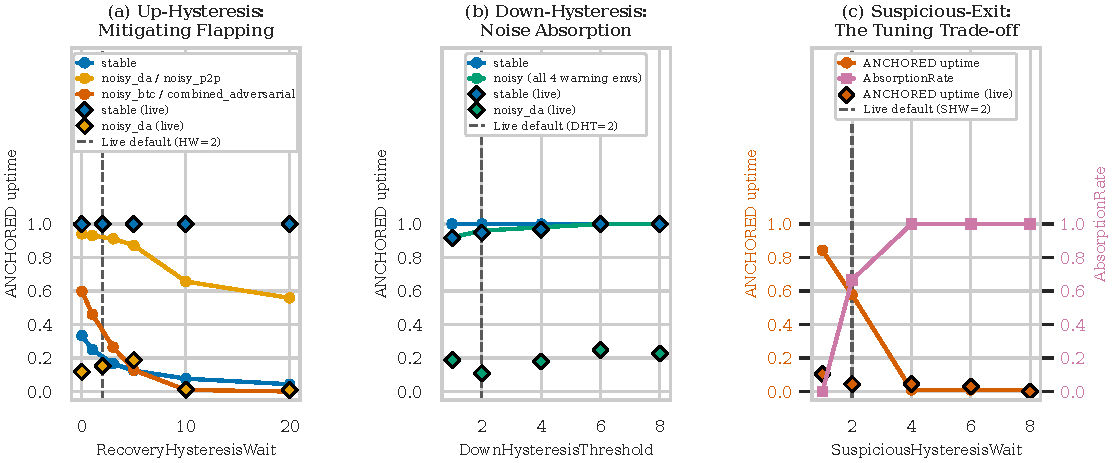
\includegraphics[width=0.95\linewidth]{figures/hysteresis_tradeoffs.pdf}
\caption{Hysteresis parameter sweep across all three absorb edges. Lines:
in-process sweep under different noise profiles; diamonds: live spot-checks
on the real 7-validator cluster (divergence from the in-process line is
real network behavior, not measurement noise); dashed line: the protocol's
live production default.}
\label{fig:hysteresis}
\end{figure}

\begin{table}[tbp]
\caption{Down-hysteresis sweep (\textsc{Anchored}$\to$\textsc{Suspicious}),
in-process (101 blocks, noise probability 0.2, seed 11, one run per threshold)}
\label{tab:hysteresis-down}
\centering
\footnotesize
\begin{tabular}{@{}lrrrrr@{}}
\toprule
\textbf{Threshold} & 1 & 2 & 4 & 6 & 8 \\
\midrule
Flapping (count)     & 5 & 1 & 1 & 0 & 0 \\
Anchored uptime (\%) & 92.08 & 96.04 & 98.02 & 100.00 & 100.00 \\
Absorption rate (\%) & 84.21 & 94.74 & 95.24 & 100.00 & 100.00 \\
\bottomrule
\end{tabular}
\end{table}

On the \textsc{Anchored}$\to$\textsc{Suspicious} edge
(Table~\ref{tab:hysteresis-down}), raising the down-hysteresis
threshold from 1 to 4 reduces flapping from 5 events to 1 and raises
anchored uptime from 92.1\% to 98.0\%, and the absorption rate rises from
84.2\% to 95.2\% and reaches 100\% at threshold 6. The live spot-check changes the conclusion. Under wide-area jitter alone,
with no injected fault, thresholds 1, 2, and 4 still flapped, and only
thresholds $\geq 6$ were clean (0 flaps, 100\% uptime). The later live runs do not
repeat this for $k{=}4$: it did not flap in the stationary sweep (one run,
Table~\ref{tab:adaptive-live}) nor in the six three-phase runs
(Table~\ref{tab:nonstationary-live}), whereas the spot-check is a single run on
one noise period, so we weigh the later runs more. The default of 2
used in the other experiments is therefore too low for WAN conditions; the
other experiments did not count flaps and cannot be taken as evidence to
the contrary. A static default must trade reaction time (low $k$) against
noise immunity (high $k$); the adaptive alternative is the exploratory extension
at the end of this section.

The other two edges show the opposite side of the trade-off. On the \textsc{Recovering}$\to$\textsc{Anchored} edge, a
larger hysteresis wait strictly reduces anchored uptime under sustained
critical-level noise (59.8\%$\to$0.0\% as the threshold goes from 0 to 20),
under the critical-level noise of Section~\ref{subsec:montecarlo}. This
follows from the design. In \textsc{Recovering}, a critical reading returns the
chain directly to \textsc{Sovereign} (the \textsc{Recovering} branch of
\texttt{CalculateNextState}), so the run of healthy blocks must start again,
and a longer wait is less likely to complete between two critical readings. On the \textsc{Suspicious}$\to$\textsc{Anchored} edge, absorption rate
rises from 0\% to 100\% as the threshold goes from 1 to 4, at a cost: the \textsc{Suspicious} timeout keeps running while the
counter accumulates, so only thresholds 1--2 reached \textsc{Anchored}
before the timeout forced \textsc{Sovereign}. Any adaptive threshold
must therefore stay below the \textsc{Suspicious} timeout, which bounds
$k_{\max}$. 


\subsection*{Discussion: griefing, history divergence and future work}

\textbf{Cost of griefing.} An adversary that degrades the peripheral view of
the honest validators -- for example by delaying their Bitcoin
connectivity -- can drive the chain into \textsc{Sovereign} and freeze
withdrawals for as long as the degradation lasts. In P4 (Section~\ref{subsec:rq1}) a sustained delay on the P2P interfaces of one validator, observed by all seven, was enough in all three runs; we did not establish whether the cause is the sensor design or a threshold crossing, so Lemma~\ref{lem:honest-range} does not prevent it. This is a new attack surface relative to a chain
that ignores its periphery, but not relative to a strict receipt-gated chain: the same
attacker stalls the strict receipt-gated chain, whereas Engram freezes only
withdrawals. Lemma~\ref{lem:honest-range} prevents Byzantine validators from causing the freeze
alone: honest validators whose peripheral view is degraded must supply the
rest of the majority. Together with the Byzantine validators they must hold
more than half of the certificate weight, and the proposer's choice of quorum
subset sets that weight. At $n{=}7$ with two colluders, an honest proposer that
includes all seven observations requires two degraded honest validators, and a
Byzantine proposer that selects a minimal quorum of five requires one.
In a design without a quorum-backed health input, one node's view
suffices. The freeze is the intended response to an
unverifiable periphery, not a safety violation. Its economic cost to users and
the attacker's cost of sustaining it are not quantified.

The analysis of repeated triggering of \textsc{Suspicious} is in Appendix~\ref{app:extended}.

\textbf{History divergence at re-anchoring.} During \textsc{Sovereign}, the
ordering of blocks rests on the validator quorum alone. A coalition
exceeding $f$ could produce a \textsc{Sovereign} history that differs from
one it would have produced under Bitcoin timestamping; the recovery proof
certifies the history's continuity, its recorded mode and lock labels, and the boundary quorum signatures. It does not
certify its uniqueness beyond the $f$ bound, that every transition followed the transition function, or that no withdrawal
executed (the lock is enforced when a block executes; the proof covers the flag recorded for it), and it does not cover the
unproven tail. The withdrawal lock limits what such a history can extract.

\textbf{Data availability of the \textsc{Sovereign} interval.} During
\textsc{Sovereign} the interval's block data is held only by the validators' own
block stores. The backfill gate of Section~\ref{subsec:reanchoring} makes its
publication a precondition for returning to \textsc{Anchored}.

\subsection{Future Work}
\label{subsec:future-work}

\begin{itemize}
  \item \emph{Formal scope.} Closing the cross-layer refinement and extending
  the certificate model from Boolean to numeric observations would extend the
  formal results to the composed system; a compositional argument for the
  interleaving of environment and consensus steps would extend the partial results
  of Section~\ref{subsec:verification-scope}. Deductive
  methods~\cite{padon2016ivy,lotan2025implicit} complement bounded model checking
  where it does not scale.
  \item \emph{Prover.} Proofs of segments built at the same time on one to four workers keep the tail within the bound
  on the cloud testbed (Section~\ref{subsec:rq3}); the aggregation of chunks proven in parallel, and
  longer intervals, are not measured. Incremental recursion would also make the recovery artifact constant-size for
  intervals of any length.
  \item \emph{Closing the tail.} Keeping the headers of the unproven tail after the return to \textsc{Anchored} and
  accepting proofs for them while the chain is \textsc{Anchored} would make every \textsc{Sovereign} and \textsc{Recovering} block
  eventually covered by a proof; it does not touch the transition function, so the specification of the FSM would not change.
  A single pending tail is implemented and unit-tested in a development branch of the repository, not evaluated end to end: a
  tail still open when the next interval begins cannot be chained to it (the \textsc{Anchored} blocks between them are not
  tracked), so that variant drops it and counts the dropped blocks. A list of pending tails, or tracking headers while the chain
  is \textsc{Anchored}, would remove the drop at a cost in state and in the analysis of the proof gate.
  \item \emph{Data availability.} Replacing single-bridge trust with sampling
  across independent peers would let the DA sensor detect partial withholding
  rather than only outages.
  \item \emph{Baselines and verifiers.} A receipt-gated baseline whose proposals
  carry verifiable evidence (a Bitcoin header chain with a Merkle proof, and a proof
  that the blob was posted) would remove the disagreement between validators of the
  out-of-band baseline, but it would still stall while a layer is down. An external
  verifier (Section~\ref{sec:protocol}), a light client or bridge on another chain
  that accepts a re-anchoring checkpoint only with a valid proof, is also unbuilt, so
  its verification cost is unmeasured.
  \item \emph{The proposer's influence on the certificate.} Requiring one observation
  in the certificate for every commit vote of \texttt{LastCommit} is a single added
  condition in \texttt{ProcessProposal}; it does not affect an honest proposer and
  makes an omission visible and attributable. The proposer would still choose which
  precommits \texttt{LastCommit} records, because CometBFT accepts any
  \texttt{LastCommit} with more than two thirds of the voting power; removing that
  choice changes the agreement protocol, needs a new safety and liveness analysis and
  would require every experiment to be run again. The quantified influence of
  Section~\ref{subsec:health-certificate} stays the guarantee of this paper.
  \item \emph{Asset-level safety.} The lock is a necessary condition for protecting
  bridged assets, not a sufficient one. It needs (i) a bridge on the counterparty
  chain that releases funds only against a proof that the Engram height is committed
  in an anchored state, with escrow accounting and replay protection; (ii) a treatment
  of history rewriting by a coalition above the fault bound while the chain is in
  \textsc{Sovereign} mode (Section~\ref{sec:protocol}); and (iii) a bound on the
  exposure before the lock, for example by a withdrawal quota per Bitcoin block. We
  evaluate none of these.
\end{itemize}

\subsection*{Additional figures and tables}

\begin{table}[tbp]
\caption{Hysteresis waits of the FSM (defaults of the prototype;
Section~\ref{subsec:transitions}).}
\label{tab:fsm-waits}
\centering
\footnotesize
\newcommand{\rcc}[1]{\raggedright\arraybackslash #1}
\begin{tabular}{@{}>{\rcc}p{0.2\linewidth}>{\rcc}p{0.34\linewidth}>{\rcc}p{0.26\linewidth}>{\rcc}p{0.1\linewidth}@{}}
\toprule
\textbf{Wait} & \textbf{Applies to} & \textbf{Default} & \textbf{Adaptive} \\
\midrule
Down wait $k_{\downarrow}$ & \textsc{Anchored}$\to$\textsc{Suspicious}, \textsc{Recovering}$\to$\textsc{Sovereign} & 2; with the optional backoff, doubles per flap level up to a cap (equal to the threshold on the testbed, so the threshold is static) & Optional \\
Suspicious exit $k_{\uparrow}$ & \textsc{Suspicious}$\to$\textsc{Anchored} & 2 (8 on the testbed) & No \\
Recovery $H$ & \textsc{Recovering}$\to$\textsc{Anchored} & 2 & No \\
\bottomrule
\end{tabular}
\end{table}

\begin{figure}[tbp]
\centering
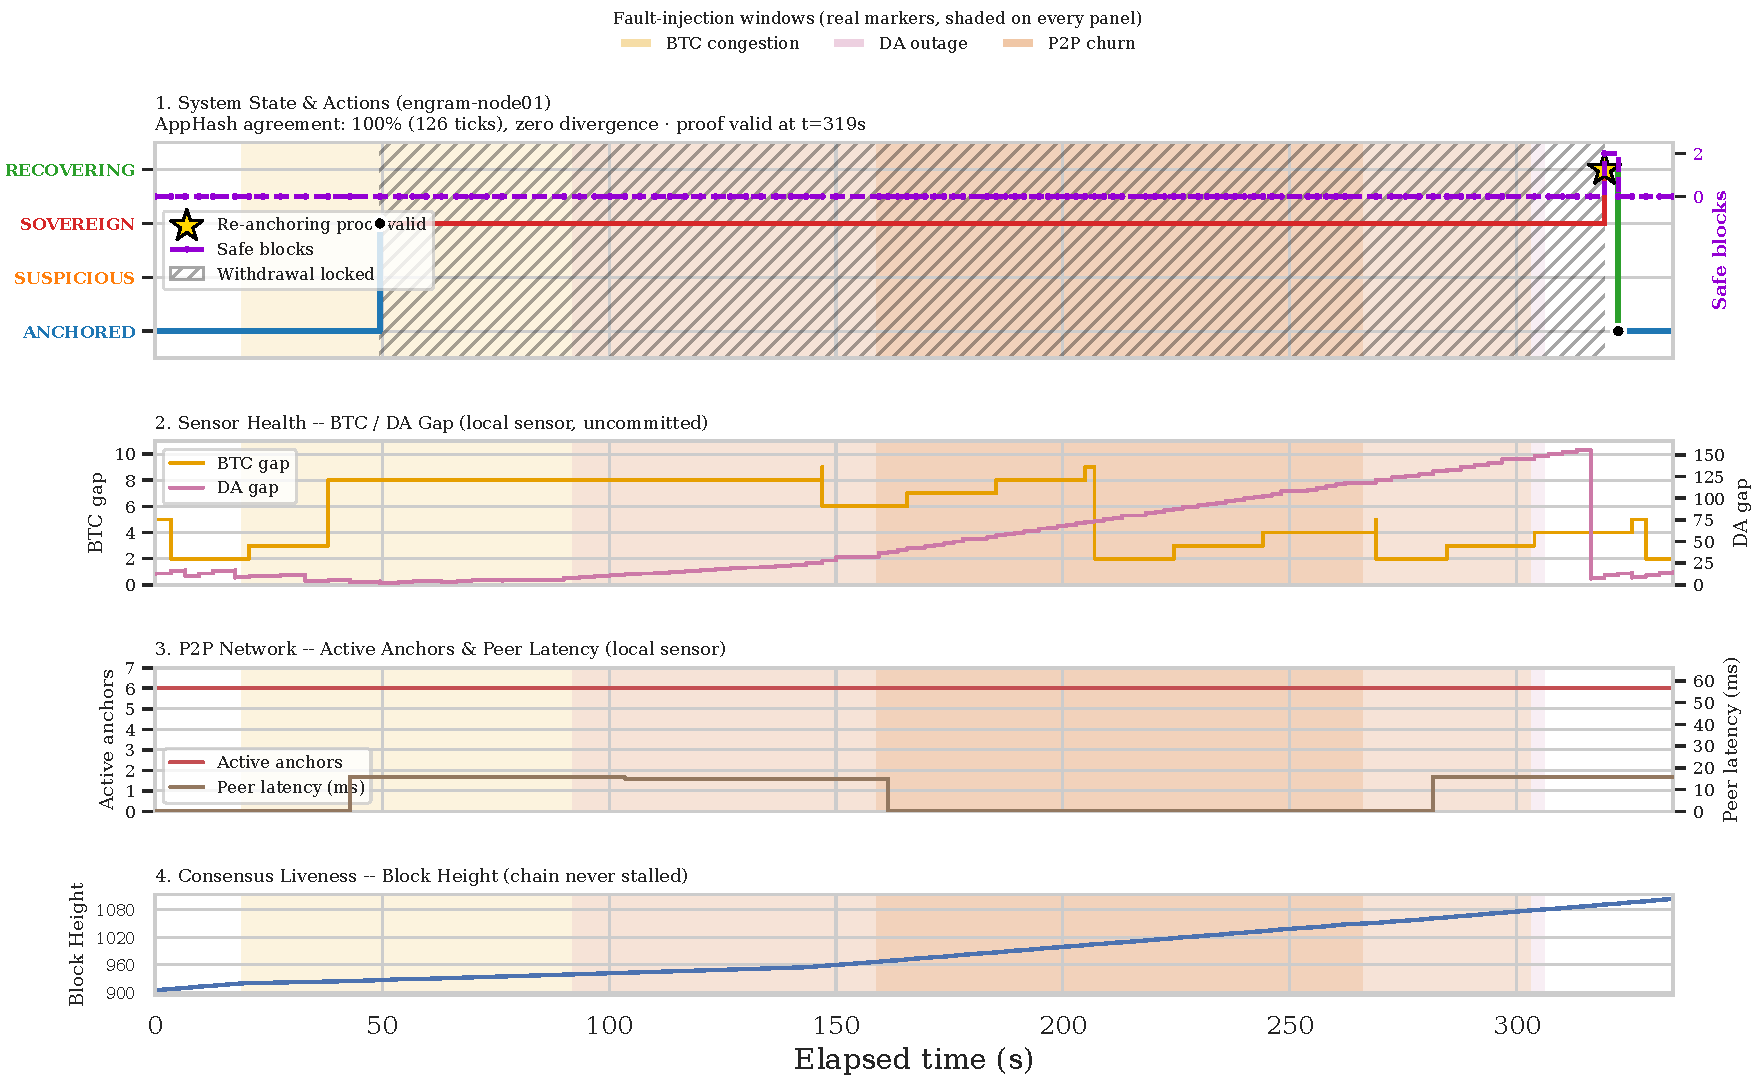
\includegraphics[width=0.95\linewidth]{figures/composite_fault_timeline.pdf}
\caption{FSM state timeline, sensor readings, P2P network state, and block
height under a layered composite fault sequence (Bitcoin congestion + DA
outage + P2P churn, overlapping at their peak). First composite run: one trial,
heuristic fallback enabled.}
\label{fig:fsm-timeline}
\end{figure}

\begin{table}[tbp]
\caption{Time from the start of a fault to the lock of withdrawals, as measured
on the testbed (Bitcoin block every 20\,s) and converted to mainnet cadence
(every 600\,s). Engram blocks are 1.2\,s on both.}
\label{tab:exposure}
\centering
\footnotesize
\begin{tabular}{@{}lrrrr@{}}
\toprule
\textbf{Fault} & \textbf{Testbed} & \textbf{Bitcoin blocks} & \textbf{Engram blocks} & \textbf{Mainnet} \\
\midrule
Checkpoint pause & 125\,s & 6.3 & 104 & 62\,min, 3{,}100 blocks \\
DA outage & 40\,s & --- & 33 & 40\,s, 33 blocks \\
\bottomrule
\end{tabular}
\end{table}


\subsection*{Methodology: baseline definitions, workloads and the Celestia setup}

\textbf{Celestia.} The DA layer is Celestia software, not the Celestia network. A private
\texttt{celestia-app} chain with one validator produces a block every 11.0\,s (median
11.0\,s, standard deviation 0.04\,s over 80 consecutive blocks; no timing parameter is set,
so this is the image default), about nine Engram blocks, and the seven bridges download
and verify its full blocks. There is no public network, no light node or data availability
sampling, and no independent operator, so a DA fault is the loss of the bridges and not the
partial withholding of data. The DA gap counts Engram heights (Section~\ref{subsec:sensors}):
its threshold of 30 blocks, about 36\,s, spans about three Celestia blocks, and a healthy chain
sits below it: in the first 15\,s of seven composite runs the gap averaged 12.3 blocks (95th
percentile 17, maximum 18; 781 samples). The lock time after a DA outage does not scale with the
Celestia cadence. The DA results therefore show
what Engram does when the DA layer is lost, not that it detects partial withholding.

\textbf{Out-of-band receipt-gated baseline (RQ2).} The same predicate and the
same pinned \textsc{Anchored} state, but the receipts are not read through the
vote extensions: in \texttt{PrepareProposal} and \texttt{ProcessProposal} each
validator reads Bitcoin and the DA layer itself and checks the proposal against
its own reading (\texttt{ENGRAM\_MODE=hard-gated-oob}). A rejected height
therefore cannot starve the next one of fresh receipts, which removes both
dependencies on block commits of the in-band baseline (Section~\ref{subsec:rq2}). The price
is that two honest validators may read different values and disagree on the
validity of a proposal, which the certificate of
Section~\ref{subsec:health-certificate} exists to prevent. It is a second
construct of this paper, built to show whether the in-band baseline's failure to
resume is a property of where the receipts are observed rather than of gating
validity on them. In what follows the first baseline is called in-band and this
one out-of-band observation; both are receipt-gated and neither locks
withdrawals.

\emph{What the predicate implies, and what RQ2 measures.} If, over an interval,
some receipt predicate holds for no proposal at any height, then no value
satisfying $V_h$ can be decided in that interval. This is the external-validity
property of Byzantine agreement~\cite{cachin2001secure}, and in CometBFT an
application rejection in \texttt{ProcessProposal} yields a nil prevote. It is a
consequence of the predicate, not a result of this paper. RQ2 therefore asks
different questions: how many blocks the implementation commits while the
predicate is nearly unsatisfiable (the receipt tolerance widens with the round),
whether it resumes after the fault, and what Engram commits instead. The
first two depend on the implementation and are reported separately for the two
variants.

\textbf{Vanilla CometBFT (control, RQ4).} The same application with the
health-aware ABCI++ hooks disabled. It does not depend on Bitcoin or
Celestia and therefore never stalls when they fail; it serves as the
cost reference for RQ4 and as a control showing that measured stalls or
fallbacks are not artifacts of the harness.

\textbf{Ablation baselines.} A peer-count-only P2P detector isolates the
contribution of the six-bound profiler (RQ1), and each hysteresis edge with
its threshold set to its floor isolates the contribution of hysteresis
(RQ3).

\textbf{Synthetic workloads.}\label{subsec:montecarlo} Two synthetic workloads feed the in-process studies; both use fixed seeds, and
Appendix~\ref{app:setup} gives the generators and their limits. The hysteresis
sweeps drive the real state machine with sensor readings in which each block is
disturbed independently with probability 0.2, for 100 blocks, so every threshold
value sees the same noise sequence. The Monte Carlo P2P study compares the
six-bound profiler with a peer-count-only rule on 2{,}000 benign and 2{,}000
full-intensity synthetic snapshots, and on ramps of rising intensity, at
production-scale thresholds; it measures false-positive and false-negative rates,
detection delay and an evasion threshold. The benign distribution, the attack
directions and the intensity scale are our choices, so the results characterize
the detectors' sensitivity within this generator.


\subsection*{Protocol: who verifies what}

\textbf{Who verifies what.} The recovery proof is submitted as a message and
verified by \emph{every Engram validator} during block execution, using an
embedded, deterministic WebAssembly build of the UltraHonk verifier. The
message handler binds the proof's public inputs to chain state:
\begin{itemize}
  \item $\mathit{rt}_{\text{last}}$ to the committed last anchored root, and
  $\mathit{rt}_{\text{new}}$ to the accumulator of a header the chain recorded;
  \item the first height to the last anchored height plus one, and the header
  count to the distance between the two checkpoints;
  \item the first and last block hashes to the CometBFT hashes the chain
  recorded at those heights, and the validator-set hash to that of the genesis
  set.
\end{itemize}
A verified height is latched so a proof cannot be replayed. Interior headers
are bound only through the accumulator, not through per-block signatures.
Bitcoin only timestamps the checkpoint; it does not verify the proof. After
recovery, validators resume writing \texttt{OP\_RETURN} checkpoints of 44 bytes
(a 4-byte tag, the Engram height, and the CometBFT block hash at that height),
and the Bitcoin gap sensor requires them to reach depth
$K_{\text{DEEP\_FINALITY}}$. Anchor re-verification compares the hash with the
local block hash. The proof's $\mathit{rt}_{\text{new}}$ is a Poseidon2
accumulator, not a block hash, and is not written to Bitcoin.

\subsection*{Related work: agreement under degraded conditions and rollup fallback}

\textbf{Agreement core.}
PBFT~\cite{castro1999pbft} and the partial-synchrony model of Dwork, Lynch,
and Stockmeyer~\cite{dwork1988consensus} underlie Tendermint and its CometBFT
successor~\cite{buchman2016tendermint,buchman2018gossip}, which provide
deterministic finality with a rotating proposer. HotStuff~\cite{yin2019hotstuff}
achieves responsiveness and linear communication under a correct leader within the same
leader-based lineage. Narwhal/Tusk~\cite{danezis2022narwhal} separate
transaction dissemination from ordering, and Bullshark~\cite{spiegelman2022bullshark}
orders transactions on top of the Narwhal DAG. These protocols agree on the content of a proposal; whether
a proposal is acceptable is decided by an application predicate that every
correct validator must evaluate identically. Tendermint's consensus problem
includes such a \texttt{valid()} predicate~\cite{buchman2018gossip}, and Cachin
et al.~\cite{cachin2001secure} introduced the \emph{external validity}
condition for multi-valued Byzantine agreement. Engram relies on the
same structure: its proposal-validation predicate depends on the health
certificate, so the predicate stays deterministic only if the certificate is
itself agreed on. BFT forensics~\cite{sheng2021forensics} studies how many malicious replicas
can be identified after a safety violation. AdoB~\cite{honore2024adob}
mechanizes benign and Byzantine consensus in one model, and
Adore~\cite{honore2022adore} adds certified reconfiguration. Engram inherits
CometBFT's evidence pool for accountability and leaves the agreement core
unchanged.

\textbf{Fast paths and protocol switching.}
A second group changes the protocol's behavior in response to conditions that
the replicas themselves observe. Abstract~\cite{aublin2015next700} lets a replicated
state machine abort a client request when something goes wrong, which supports
composing and reconfiguring BFT protocols. Thunderella~\cite{pass2018thunderella} combines an
optimistic fast path with a synchronous fallback, and
Autobahn~\cite{giridharan2024autobahn} targets seamless recovery from network
blips. The trigger in each case is a fault of the replicas or of the network
among them.

\textbf{Availability--finality trade-offs.}
The closest conceptual relatives give up finality to keep the chain growing.
The sleepy model~\cite{pass2017sleepy} lets players be online or offline and
gives a consensus protocol that is resilient as long as a majority of the online
players are honest.
Ebb-and-flow protocols~\cite{neu2021ebbflow} expose both a dynamically
available ledger and a finalized prefix, so the chain keeps growing when
finality stalls and the finalized ledger catches up on recovery. Casper
FFG~\cite{buterin2017casper}, and Gasper~\cite{buterin2020gasper}, which
combines it with the LMD GHOST fork-choice rule, prove accountable safety and
plausible liveness. For the case in which more than a third of the validators
crash, Casper FFG proposes an inactivity leak that drains the deposits of
non-voting validators until the voting validators again form a supermajority,
and leaves the exact formula open. These designs share the
``degrade, do not halt'' goal and the tension described by the CAP
theorem~\cite{gilbert2002cap}. They differ from Engram in two respects: the
trigger is \emph{internal} participation, and the response changes how finality
is reached, not which blocks and withdrawals are valid.

\textbf{Rollup fallback and its decision locus.}
When a rollup operator stops building blocks or proposing state roots, escape
hatches~\cite{figueira2025escapehatch} let users withdraw on the
L1 by proving their assets against an L2 state root. Arbitrum~\cite{kalodner2018arbitrum} resolves disputes about contract behavior
with a challenge-based protocol on the L1. Surveys of layer-two
protocols~\cite{gudgeon2020sok} treat the ability of honest users to withdraw as
a core security property, and list among the open weaknesses that layer-two
designs assume the underlying blockchain eventually accepts transactions.
Capretto et al.~\cite{capretto2025secure} give fraud-proof games,
mechanized in Lean~4, with which an honest agent can prove on the L1 that a
sequencer-and-DAC ``arranger'' violated a safety property even if all of its
replicas are compromised; a liveness violation that preserves safety cannot be
proved on the L1. A follow-up decentralizes the sequencer and the DA committee
with set consensus~\cite{capretto2026setconsensus}.

Two designs define a protocol-level response to a DA failure. AnyTrust
normally relies on a data-availability committee. If the
sequencer cannot collect enough committee signatures within a few minutes, it
posts the full data to the parent chain as a non-AnyTrust rollup would
do~\cite{arbitrum_anytrust}. Withdrawals then incur the delay of a standard
rollup, and the chain switches back to the cheaper mode when the committee
resumes~\cite{arbitrum_orbit_anytrust}. The sequencer makes this decision, and the
failure it reacts to is a committee failure. OP Stack Alt-DA keeps data with an
external DA provider and lets anyone challenge a commitment on the L1. If the
data is not posted before the resolve window elapses, derivation reorgs the
L2 blocks that depended on it~\cite{optimism_altda}. This design answers the same
question as Engram, what happens when an external DA input fails, by
resolving the failure on the L1 and discarding the affected blocks.

These designs show that protocol-defined fallback for DA and sequencing
failures exists. They differ from Engram in three respects:
\begin{itemize}
  \item \emph{Who decides.} A sequencer, a committee, users, or an L1 contract;
  Engram decides inside the validator set's own consensus instance.
  \item \emph{What is observed.} A committee or data-posting failure, not the
  health of Bitcoin settlement or of an external DA network; Engram uses signed
  observations of all three peripheral layers.
  \item \emph{What the response changes.} It publishes more data or
  reorganizes the chain; Engram changes the validity predicate and the
  withdrawal policy and commits the FSM state in the same block.
\end{itemize}


\subsection*{Formal analysis: model-checked properties and attack resilience}

\label{subsec:formal-invariants}

Six safety properties are specified. The first five are checked in the FSM safety
run (the first as an invariant, the others as action or temporal properties). The
sixth, Monotonicity Safety, is defined in the server layer and appears only in its
refinement drivers, whose runs did not complete.
\begin{itemize}
  \item \emph{Circuit Breaker Isolation:} withdrawals are locked if and only
  if the state is \textsc{Sovereign} or \textsc{Recovering}.
  \item \emph{Hysteresis Integrity:} \textsc{Recovering}$\to$\textsc{Anchored}
  requires the full hysteresis wait and a valid recovery proof.
  \item \emph{Suspicious-Exit Hysteresis Integrity:} the corresponding guard
  on \textsc{Suspicious}$\to$\textsc{Anchored}.
  \item \emph{Strict FSM Transition Safety:} only transitions drawn in
  Fig.~\ref{fig:fsm} occur.
  \item \emph{Sovereign-Data Publication:} every
  \textsc{Recovering}$\to$\textsc{Anchored} transition occurs with the DA
  backfill condition true.
  \item \emph{Monotonicity Safety:} heights and time never decrease.
\end{itemize}
The Tendermint driver checks a separate invariant covering, among others, agreement on the decided value, external validity, accountability and the absence of double spending across modes.
Five attack-specific properties are enforced by the validity predicate:
resistance to data withholding; resistance to forged or reorganized anchors
through anchor re-verification; a deterministic bound on Byzantine
timeout flooding; resistance to eclipse-driven recovery through the
six-bound P2P gate; and accountability, i.e.\ any safety violation implies
double-signing evidence. Accountability is inherited from CometBFT's
equivocation evidence pool rather than proved anew. The ablation study below tests two of them,
data withholding and eclipse-driven recovery, by removing the mechanism that
enforces each; the others are design properties of the validity predicate that
Section~\ref{sec:evaluation} exercises with fault and attack injection. All of
these properties are conditional on the Bitcoin reorg-depth bound of
Section~\ref{subsec:threat-model}.

How the server layer models the health certificates is described in Appendix~\ref{app:extended}.

